\documentclass[12pt,a4paper]{article}
\usepackage[utf8]{inputenc}
\usepackage[french]{babel}
\usepackage[T1]{fontenc}
\usepackage{amsmath}
\usepackage{amsfonts}
\usepackage{amssymb}
\usepackage{graphicx}
\usepackage{url}
\author{\textsc{TRAN Quoc Nhat Han} - \textsc{Amine MOUSTATIH}}
\title{Recherche documentaire de tests d'adéquation}
\date{\today}
\begin{document}
\maketitle 
\renewcommand{\contentsname}{Sommaire}
\tableofcontents

\clearpage

\begin{abstract}
Ce rapport est un petit recherche documentaire concernant quelques tests d'adéquation usuels:
\begin{itemize}
\item Test du $\chi^2$
\item Test de Shapiro-Wilk
\item Test d'Anderson Darling
\end{itemize}
\end{abstract}

\clearpage

\section{Test $\chi^2$}

\subsection{Histoire en bref}
Le test du $\chi^2$ (prononcé \emph{khi deux} ou \emph{khi carré}) fournit une méthode pour déterminer la nature d'une répartition, qui peut être continue ou discrète.

\subsection{Processus}
À la base d'un test de statistique classique, il y a la formulation d'une hypothèse appelée hypothèse nulle (ou hypothèse zéro), notée $H_0$. Elle suppose que les données considérées proviennent de variables aléatoires suivant une loi de probabilité donnée, et l'on souhaite tester la validité de cette hypothèse.

\begin{enumerate}
\item On répartit les valeurs de l'échantillon (de taille $n$) dans $k$ classes distinctes et on calcule les effectifs de ces classes. Il faut vérifier que pour les $i$ de $1$ à $k$, les effectifs théoriques dans chacune des classes soient au moins égal à $5$ (éventuellement répartir les valeurs autrement). Appelons $o_i$ $(i=1,...,k)$ les effectifs observés et $e_i$ les effectifs théoriques.
\item Calculer \[Q = \sum\limits_{i = 1}^k {\frac{{{{\left( {{o_i} - {e_i}} \right)}^2}}}{{{e_i}}}} \]
La statistique $Q$ donne une mesure de l'écart existant entre les effectifs théoriques attendus et ceux observés dans l'échantillon. En effet, plus $Q$ sera grand, plus le désaccord sera important. La coïncidence sera parfaite si $Q=0$.
\item On compare ensuite cette valeur $Q$ avec une valeur $\chi_{k-1, \alpha}^2$ issue d'un tableau (voir extrait ci-contre) à la ligne $k-1$ et à la colonne $a$. $\nu = k-1$ est le nombre de degrés de liberté et a la tolérance.
\begin{figure}[!h]
\centering
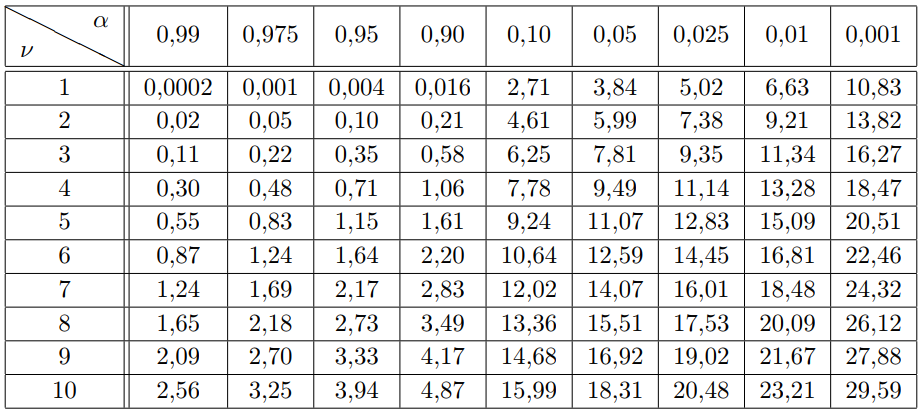
\includegraphics[width=0.8\textwidth]{images/Chi_deux.png}
\caption{Table de la loi $\chi^2$ pour $K \sim \chi^2(\nu)$ et $\alpha$ tel que $P(K \geq \chi_{\nu, \alpha})^2 = \alpha$}
\label{ChiDeux}
\end{figure}
\item Si $Q > \chi_{k-1, \alpha}^2$, et si $n$ est suffisamment grand, alors l'hypothèse d'avoir effectivement affaire à la répartition théorique voulue est à rejeter avec une probabilité d'erreur d'au plus $\alpha$.
\end{enumerate}

\subsection{Exemple}
On a lancé un dé $90$ fois et on a obtenu les issues $1$ à $6$ $(k=6)$ avec les effectifs suivants: $12, 16, 20, 11, 13, 18$ (on a vérifié que $90$ lancers sont suffisants: $n * \frac{1}{6} * \frac{5}{6} \geq 5$ implique que $n \geq 36$).
 
Si le dé n'est pas pipé (notre hypothèse), on attend comme effectifs moyens théoriques $15$ pour toutes les issues.

\begin{align*}
Q & = \frac{{{{\left( {12 - 15} \right)}^2}}}{{15}} + \frac{{{{\left( {16 - 15} \right)}^2}}}{{15}} + \frac{{{{\left( {20 - 15} \right)}^2}}}{{15}} +\\
& + \frac{{{{\left( {11 - 15} \right)}^2}}}{{15}} + \frac{{{{\left( {13 - 15} \right)}^2}}}{{15}} + \frac{{{{\left( {18 - 15} \right)}^2}}}{{15}} = \frac{{64}}{{15}} = 4,266
\end{align*}

Pour $\nu = k-1=5$ degrés de liberté et un seuil de tolérance de $5\%$, la valeur $\chi_{\nu, \alpha}$ du tableau \eqref{ChiDeux} est $11,07$. Cela signifie que la probabilité que $Q$ soit supérieur à $11\geq 1$ est de $5\%$ (voir figure \eqref{ChiDeuxExemple} ci-dessous). Comme $4,266 < 11,1$, on accepte l'hypothèse selon laquelle le dé est régulier.

\begin{figure}[!h]
\centering
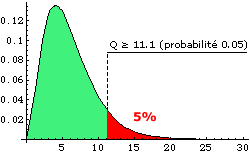
\includegraphics[width=0.5\textwidth]{images/Chi_deux_exemple.png}
\caption{Fonction de répartition de la loi du khi deux pour 5 degrés de libertés}
\label{ChiDeuxExemple}
\end{figure}

\subsection{Test MATLAB}
\begin{enumerate}
\item Créez un objet de la distribution de probabilité normale standard. Générer un vecteur $x$ de $100$ valeurs selon de la distribution.
\begin{verbatim}
pd = makedist('Normal');
x = random(pd,100,1);
\end{verbatim}
\item Tester l’hypothèse nulle que les données en $x$ proviennent d’une population avec une distribution normale.
\begin{verbatim}
h = chi2gof(x)
\end{verbatim}
\texttt{chi2gof(x)} retourne une décision de test de l’hypothèse nulle que les données de vecteur $x$ provient d’une distribution normale avec une moyenne et la variance estimée à partir de $x$, en utilisant le test du $\chi^2$ d’ajustement. L’autre hypothèse est que les données ne provient pas d’une telle distribution. Le résultat de $h$ est $1$ si le test rejette l’hypothèse nulle au seuil de signification de $5\%$ et $0$ sinon.

\begin{figure}[!h]
\centering
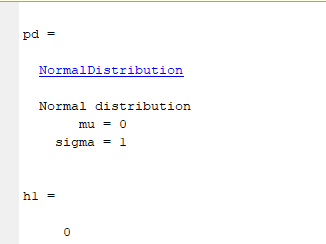
\includegraphics[width=0.5\textwidth]{images/Chi_deux_test.png}
\caption{Résultat de test $\chi^2$ en MATLAB}
\label{ChiDeuxExemple}
\end{figure}
\end{enumerate}
\clearpage
\section{Test de Shapiro-Wilk}

\subsection{Histoire en bref}
Ce test non-paramétrique est publié en 1965 par \emph{Samuel Sanford Shapiro} et \emph{Martin Wilk} pour tester si un échantillon d'une variable \textbf{continue} (sous 2000 observations) suit \textbf{une loi normale}.

\subsection{Processus}

Soit une variable continue $X$ dont $n$ observations étaient réalisées $x_1, x_2, ..., x_n$.

Soient 2 hypothèses: 
\begin{itemize}
\item $H_0$: $X$ suit une loi normale $N(\mu, \sigma^2)$.
\item $H_1$: $X$ ne suit pas la loi normale.
\end{itemize}

Nous effectuons le test comme suivant:
\begin{enumerate}
\item Ordonner les réalisations dans l'ordre croissant $y_1 \leq y_2 \leq ... \leq y_n$.
\item Calculer \[{S^2} = \sum\limits_1^n {{{\left( {{y_i} - \overline y } \right)}^2}}  = \sum\limits_1^n {{{\left( {{x_i} - \overline x } \right)}^2}} \]
Donc $\overline y, \overline x$ désignent la moyenne de $y, x$ respectivement.
\item Calculer des différences (entre le premier $y_1$ et le dernier $y_n$, le deuxième $y_2$ et l'avant-dernier $y_{n-1}$, et ainsi la suite, le médian $y_{k+1}$ est ignoré si $n=2k+1$). Appliquer un coefficient de pondérer lu dans la table \ref{ShapiroWilkTablePonderer}. Les additionner et élever au carré.
\[{b^2} = {\left( {\sum\limits_1^{\left\lfloor {\frac{n}{2}} \right\rfloor } {{a_i}\left( {{y_{n + 1 - i}} - {y_i}} \right)} } \right)^2}\]
\begin{figure}[!h]
\centering
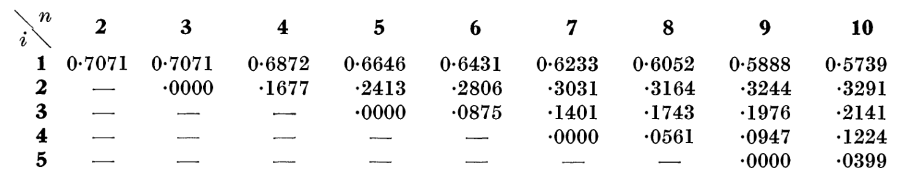
\includegraphics[width=\textwidth]{images/ShapiroWilk_N_1_10.png}
\caption{Coefficients $a_{n+1-i}$ pour $n=1..10$}
\label{ShapiroWilkTablePonderer}
\end{figure}
\item Calculer le statistique du test \[W = \frac{{{b^2}}}{{{S^2}}}\]
\item Rechercher la valeur $W$ dans la table \ref{ShapiroWilkTablePourcentage}. Petit $W$ signifie une distribution non normale.
\begin{figure}[!h]
\centering
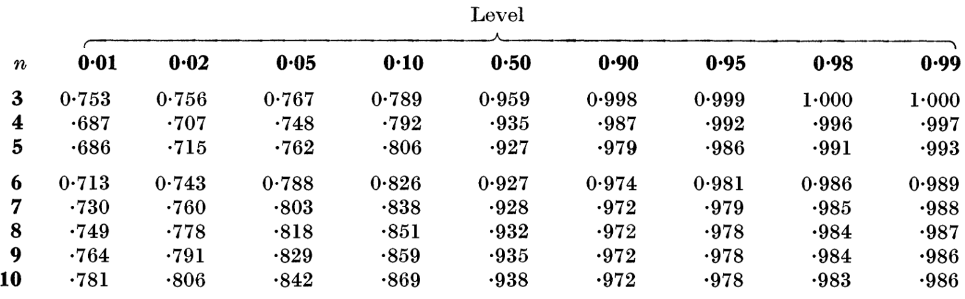
\includegraphics[width=\textwidth]{images/ShapiroWilk_Percentage.png}
\caption{Pourcentage de $W$ pour $n=1..10$}
\label{ShapiroWilkTablePourcentage}
\end{figure}
Choisir la valeur plus proche à $W$ dans la ligne correspondant à $n$. Regarder alors le niveau (\emph{level}) de signifiance $p-value$. Si $p-value > \alpha$ ($\alpha$ est le risque, souvent $1\%$ ou $5\%$), l'hypothèse $H_0$ est accepté.
\end{enumerate}
\subsection{Code en R}
\begin{verbatim}
shapiro.test(x)
\end{verbatim}

$x$ désigne un vecteur de données.

\subsubsection*{Exemples}
\begin{verbatim}
> shapiro.test(rnorm(100, mean = 5, sd = 3))

Résultat de la commande:

Shapiro-Wilk normality test

data: rnorm(100, mean = 5, sd = 3)
W = 0.9895, p-value = 0.6211
\end{verbatim}

$p$ est significativement plus grand que $\alpha=5\%$. L'hypothèse nulle est donc non rejetable.

\begin{verbatim}
> shapiro.test(runif(100, min = 2, max = 4))

Résultat de la commande:
Shapiro-Wilk normality test

data: runif(100, min = 2, max = 4)
W = 0.9337, p-value = 8.077e-05
\end{verbatim}

$p$ est trop faible. L'échantillon, par conséquence, ne suit pas la loi normale.

\section{Anderson Darling}
\subsection{Histoire en bref}
Inventé par \emph{Theodore Wilbur Anderson} (1918–2016) et \emph{Donald A. Darling} (1915–2014) le 1952, ce test est pour but de vérifier si un échantillon est issu d'une loi \textbf{continu} donnée. Quoi qu'il est similaire au test Kolmogorov-Smirnov, il fait beaucoup plus attention au \textbf{queue} de la courbe de la fonction de distribution en tenant compte la loi à vérifier dans le formule. C'est pourquoi les valeurs critiques dépendent de la loi à vérifier.

Ce test peut se généraliser pour tester la vraisemblance entre une famille de distribtion (la fonction de répartition n'est pas forcément spécifiée), ou estimer les paramètres.

\subsection{Processus}
Soit une variable continue $X$ dont $n$ observations étaient réalisées $x_1, x_2, ..., x_n$.

Soient 2 hypothèses: 
\begin{itemize}
\item $H_0$: $X$ suit une loi dont $F(x)$ est la fonction de distribution cumulative. Les paramètres de $F$ sont connus.
\item $H_1$: $X$ ne suit pas la loi normale.
\end{itemize}

Nous effectuons le test comme suivant:
\begin{enumerate}
\item Ordonner les réalisations dans l'ordre croissant $y_1 \leq y_2 \leq ... \leq y_n$.
\item Calculer le statistique du test
\[{A^2} =  - n - \sum\limits_{i = 1}^n {\frac{{2i - 1}}{n}\left( {\ln F\left( {{Y_i}} \right) + \ln \left( {1 - F\left( {{Y_{n + 1 - i}}} \right)} \right)} \right)} \]
\item Comparer $A$ avec les valeurs critiques de la loi à vérifier. Si $A$ est supérieur, l'hypothèse $H_0$ est rejeté. Autrement, on regarde le $p-value$.
\end{enumerate}

\subsection{Code en R}
Il faut utiliser le package \emph{nortest}.

\begin{verbatim}
library(nortest)
ad.test(x)
\end{verbatim}

$x$ est le vecteur de données.

\subsubsection*{Exemples}
\begin{verbatim}
set.seed(403)
y1 = rnorm(n, mean = 0, sd = 1)
ad.test(y1)

>         Anderson-Darling normality test
>
> data:  y1 
> A = 0.3093, p-value = 0.5568
\end{verbatim}
Avec $\alpha = 0.05 < p-value$, nous acceptons $H_0$.

\begin{verbatim}
set.seed(403)
y2 = rexp(n,rate=1) - rexp(n,rate=1)
ad.test(y2)

>         Anderson-Darling normality test
>
> data:  y2 
> A = 13.6652, p-value < 2.2e-16
\end{verbatim}
Avec $\alpha = 0.05 > p-value$, nous rejetons $H_0$.
\begin{thebibliography}{3}
\bibitem{ShapiroWilk}

S. S. Shapiro et M. B. Wilk, \emph{An analysis of variance test for normality (complete samples)}

\url{https://github.com/haghish/ST516/blob/master/Articles/Shapiro-Wilks%20test/An%20analysis%20of%20variance%20test%20for%20normality%20(complete%20samples).pdf}

\bibitem{TestsNormalite} 
\url{http://www.jybaudot.fr/Inferentielle/testsnormalite.html}

\bibitem{ShapiroWilkR}
\url{http://www.sthda.com/french/wiki/test-de-normalite-avec-r-test-de-shapiro-wilk}

\bibitem{ShapiroWilkRex}
\url{https://stat.ethz.ch/R-manual/R-patched/library/stats/html/shapiro.test.html}

\bibitem{AndersonDarlingWiki}
\url{https://en.wikipedia.org/wiki/Anderson%E2%80%93Darling_test}

\bibitem{AndersonDarlingHandbook}
\url{https://itl.nist.gov/div898/handbook/eda/section3/eda35e.htm}

\bibitem{TablesValeurs}
Christophe Chesneau, \emph{Tables de valeurs}

\url{https://chesneau.users.lmno.cnrs.fr/tables-valeurs.pdf}
\end{thebibliography}
\end{document}